\documentclass{article}
\usepackage[utf8]{inputenc}
\usepackage[cm]{fullpage}
%\usepackage[spanish,mexico]{babel}

\usepackage{siunitx}
\sisetup{
	output-complex-root = \ensuremath{\mathrm{j}},
	complex-root-position = before-number
}

\usepackage[inline]{enumitem}

\usepackage{graphicx}
%\usepackage{wrapfig}
\usepackage{hyperref}
\usepackage{datatool}



\usepackage{tabularx}
\usepackage[table]{xcolor}
\usepackage{multirow}
\usepackage{hhline}


\definecolor{Gray}{gray}{0.85}
\definecolor{LightCyan}{rgb}{0.88,1,1}

\newcommand{\Subject}{Circuit analysis II}
\newcommand{\Group}{5A}
\newcommand{\Carrera}{Electrical engineering}
\newcommand{\ExamType}{Exam 1 (Max time: One and half hours)}
\newcommand{\Date}{7/10/2016}
\newcommand{\MaximumMarks}{10}
\newcommand{\PName}{Dr. Suresh Kumar Gadi}


\makeatletter
% Blank/missing fields commands
% \skipblank adds \\ to filled field; * version adds \space instead of newline
\newcommand\skipblank{\@ifstar\@spskip\@nlskip}
\newcommand\@nlskip[1]{\ifthenelse{\DTLiseq{#1}{}}{\relax}{#1\\}}
\newcommand\@spskip[1]{\ifthenelse{\DTLiseq{#1}{}}{\relax}{#1\space}}
% \checkblank replaces blank fields with ***
\newcommand\checkblank[1]{\ifthenelse{\DTLiseq{#1}{}}{***}{#1}}
\makeatother

\begin{document}
	\linespread{2.5}
	\DTLloaddb{addresses}{db/questions.csv} % use your actual address database here
	\DTLforeach*{addresses}{%
		\VarOOA  =VarOOA,
		\VarOOB  =VarOOB,
		\VarOOC  =VarOOC,
		\VarOOD  =VarOOD,
		\VarOOE  =VarOOE,
		\VarOOF  =VarOOF,
		\VarOOG  =VarOOG,
		\VarOOH  =VarOOH,
		\VarOOI  =VarOOI,
		\VarOOJ  =VarOOJ,
		\VarOOK  =VarOOK,
		\VarOOL  =VarOOL,
		\VarOOM  =VarOOM,
		\VarOON  =VarOON,
		\VarOOO  =VarOOO,
		\VarOOP  =VarOOP,
		\VarOOQ  =VarOOQ,
		\VarOOR  =VarOOR,
		\VarOOS  =VarOOS,
		\VarOOT  =VarOOT,
		\VarOOU  =VarOOU,
		\VarOOV  =VarOOV,
		\VarOOW  =VarOOW,
		\VarOOX  =VarOOX,
		\VarOOY  =VarOOY,
		\VarOOZ  =VarOOZ,
		\VarOOa  =VarOOa,
		\VarOOb  =VarOOb,
		\VarOOc  =VarOOc,
		\VarOOd  =VarOOd,
		\VarOOe  =VarOOe,
		\VarOOf  =VarOOf,
		\VarOOg  =VarOOg,
		\VarOOh  =VarOOh,
		\VarOOi  =VarOOi,
		\VarOOj  =VarOOj,
		\VarOOk  =VarOOk,
		\VarOOl  =VarOOl,
		\VarOOm  =VarOOm,
		\VarOOn  =VarOOn,
		\VarOOo  =VarOOo,
		\VarOOp  =VarOOp,
		\VarOOq  =VarOOq,
		\VarOOr  =VarOOr,
		\VarOOs  =VarOOs,
		\VarOOt  =VarOOt,
		\VarOOu  =VarOOu,
		\VarOOv  =VarOOv,
		\VarOOw  =VarOOw,
		\VarOOx  =VarOOx,
		\VarOOy  =VarOOy,
		\VarOOz  =VarOOz,
		\SName =Name,
		\No =No}
	{%
		\setcounter{page}{1}
		%\thispagestyle{empty}
		\begin{center}
			\begin{minipage}{.15\textwidth}
				\begin{flushleft}
					
\includegraphics[width=\textwidth]{images/uadec-original}
				\end{flushleft}
			\end{minipage}
			\begin{minipage}{.84\textwidth}
				\begin{flushright}
					{\Huge \textbf{Universidad Autónoma de Coahuila}}\\[2mm]
					{\huge Facultad de Ingeniería Mecánica y Eléctrica}\\[2mm]
					{\LARGE Unidad Torreón}
				\end{flushright}
			\end{minipage}
		\end{center}
		%\\[0.5cm]
		\begin{center}
			\setlength\doublerulesep{2pt}\doublerulesepcolor{LightCyan}
			\begin{tabularx}{\textwidth}{ ||>{\columncolor{Gray}}l|X||>{\columncolor{Gray}}l|r|| }
				\hhline{|t==:t:==t|}
				Subject      		& \Subject  		& Group         	& \Group   					\\ \hhline{|:==::==:|}
				Degree         		& \Carrera  		& Date      		& \Date     				\\ \hhline{|:==::==:|}
				Exam / Homework		& \ExamType    		& Registration \#	& \textbf{\textit{\No}}       				\\ \hhline{|:==::==:|}
				Professor's name	& \PName			& Marks Obtained	& \underline{\hspace{1cm}} $\Big /10$				\\ \hhline{|:==:b:==:|}
				Student's name		& \multicolumn{3}{X||}{\textbf{\textit{\MakeUppercase{\SName}}}}	\\ \hhline{|b====b|}
			\end{tabularx}
		\end{center}
		\section*{Instructions}
		\begin{enumerate}
			\item In the calculations, the student should maintain at least a precision of 3 decimal places with a correct rounding. (20\% of the marks obtained will be reduced)
		\end{enumerate}
		\section*{Questions}
		\begin{enumerate}
			\item  Let $Z_1=\SI{-j{\VarOOA}}{\ohm}$, $Z_2=\SI{+j{\VarOOB}}{\ohm}$, $Z_3=\SI{{\VarOOC}}{\ohm}$, $Z_4=\SI{{\VarOOD}}{\ohm}$, $Z_5=\SI{{\VarOOE}}{\ohm}$, $Z_6=\SI{{\VarOOF}+j{\VarOOG}}{\ohm}$, $V_1=\SI{{\VarOOH}}{\volt}$ and $V_2=\SI{{\VarOOI}+j{\VarOOJ}}{\volt}$. Find the current and votage across each element in the circuit shown in Figure 1.  (5 points)
			\item Calculate root mean square and average rectified value for the output voltage shown in Figure 2. (5 points)\\
			\begin{minipage}{.30\textwidth}
				\centering
				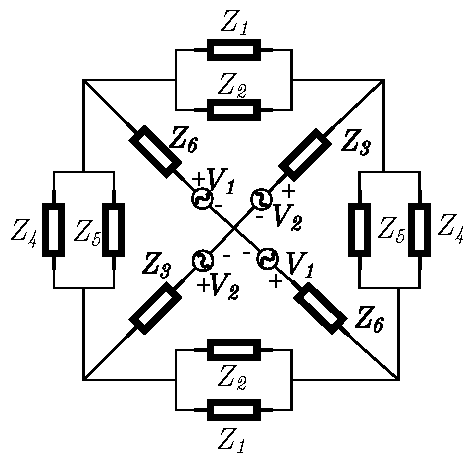
\includegraphics[height=4cm]{images/Drawing1}\\
				\textbf{Figure 1}
			\end{minipage}
			\begin{minipage}{.70\textwidth}
				\centering
				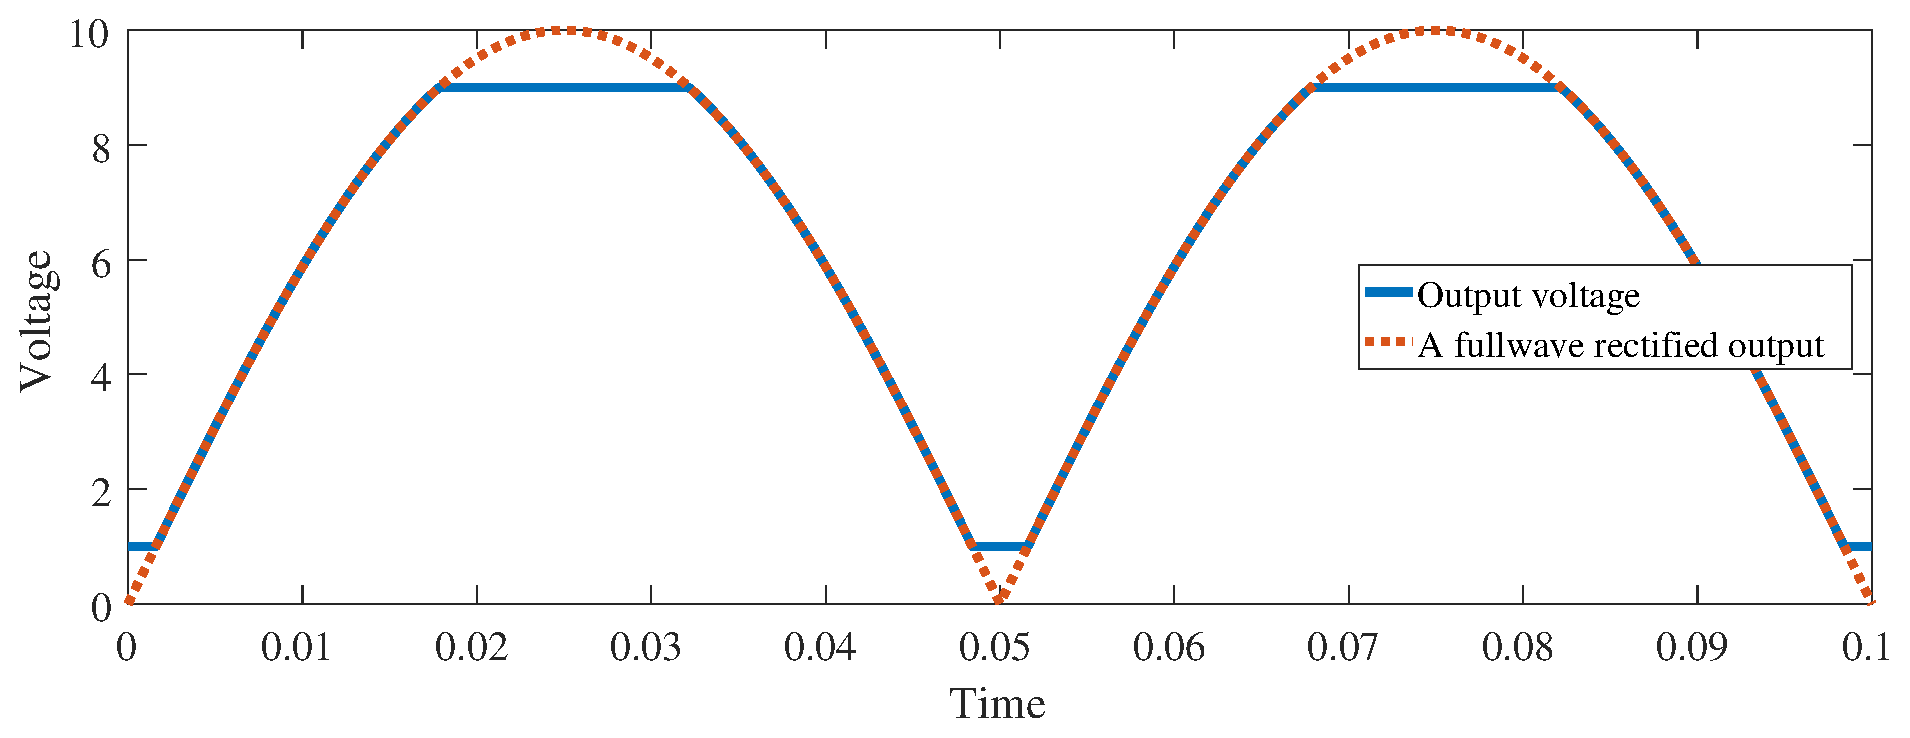
\includegraphics[height=4cm]{images/WaveForms}\\
				\textbf{Figure 2}
			\end{minipage}
			\item Calculate the impedance between the terminals shown in Figure 3. The impedance of individual element shown in the circuit is $Z=\SI{{\VarOOK}+j{\VarOOL}}{\ohm}$.  (5 points)\\
			\begin{center}
				\begin{minipage}{.70\textwidth}
					\centering
					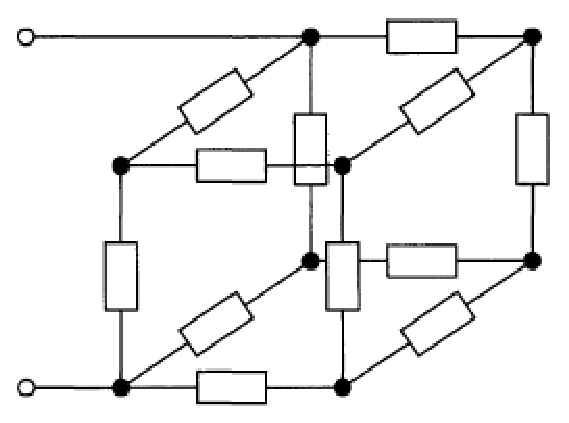
\includegraphics[height=3cm]{images/CubeImp}\\
					\textbf{Figure 3}
				\end{minipage}
			\end{center}
			\item At our school's washroom, if you drop a bubblegum or a paper in the men's urinals, what happens to it? (1 point)
		\end{enumerate}
				
		
		\clearpage
	}
\end{document}
